\documentclass[phd]{ntuthesis}

\usepackage{times}
\usepackage{verbatim}
\usepackage{color}
\usepackage{url}
\usepackage{graphicx}
\usepackage{array}
\usepackage{wallpaper} 
\usepackage{hyperref}
\usepackage{booktabs}
\usepackage{minted}

% Using the tex-text mapping for ligatures etc.
\defaultfontfeatures{Mapping=tex-text}

% Set the default fonts
\setmainfont{Times New Roman}
% \setCJKmainfont{標楷體}

\ifdefined\withwatermark
  \CenterWallPaper{0.174}{watermark.pdf}
  \setlength{\wpXoffset}{6.1725cm}
  \setlength{\wpYoffset}{10.5225cm}
\fi

% digital object identifier
\ifdefined\withdoi
  \insertdoi
\fi

\makeatletter
\AtBeginDocument{
  \hypersetup{
    pdftitle={\@titleen},
    pdfauthor={\@authoren},
    pdfsubject={\@typeen{} \@classen},
    pdfkeywords={\@keywordsen}
  }
}
\makeatother

% Your information goes here
% author: Tz-Huan Huang [http://www.csie.ntu.edu.tw/~tzhuan]

% ----------------------------------------------------------------------------
% "THE CHOCOLATE-WARE LICENSE":
% Tz-Huan Huang wrote this file. As long as you retain this notice you
% can do whatever you want with this stuff. If we meet some day, and you think
% this stuff is worth it, you can buy me a chocolate in return Tz-Huan Huang
% ----------------------------------------------------------------------------

% Syntax: \var{English}{Chinese}
\university{National Taiwan University}{國立臺灣大學}
\college{College of Electrical Engineering and Computer Science}{電機資訊學院}
\institute{Department of Computer Science and Information Engineering}{資訊工程學系}
%TODO: mention IoT in the title, might be good for ARC application
\title{CapeVM: A Fast and Safe VM for Sensor Nodes}{開普敦VM}
\author{Niels Reijers}{賴爾思}
\studentid{D00922039}
\advisor{Professor Chi-Sheng Shih}{施吉昇 教授}
\defenseyear{2018}{107}
\defensemonth{March}{3}
\defenseday{28}
\doi{doi:10.6342/NTU2017XXXXX}
\keywords{keyword}{關鍵字}


\begin{document}

\frontmatter

\makecover

\makecertification

\begin{acknowledgementsen}
I'm glad to thank\ldots 
\end{acknowledgementsen}

Abstract goes here

\tableofcontents
\listoffigures
\listoftables

\mainmatter

% Your thesis goes here
\chapter{Introduction}
to do

\chapter{Background}

\chapter{Related work}

\chapter{VM design}

\chapter{Performance optimisation}
to do

\chapter{Guaranteeing safety}

With some exceptions \cite{Evers:2010ur}, most current sensor node VMs don't discuss safety, but instead focus on the functionality provided and how this can be implemented on a tiny sensor node. This is unfortunate, because the ability to provide a safety execution environment is both desirable, and easier to implement using a VM than it is using native code.

\section{Native code approaches}
For desktop applications, Wahbe et al. described software fault isolation \cite{Wahbe:1994cj} techniques that can be used for situations where we want to isolate a piece of code without incurring the overhead of using processes and the CPU's memory protection. For example, for plugin code that frequently needs to interact with an application, the overhead of frequent context switches, but should still be isolated from the rest of the application. Two basic methods are described: we can either rewrite the native code at load time, and insert checks at all potentially unsafe writes, or we can compile the code to a more restricted format with the appropriate checks already in place, and only verify the code adheres to this standard at load time.

On a sensor node, two systems exist that follow each of these two approaches. \emph{t-kernel} \cite{Gu:2006ww} raises the level of system abstraction for the developer by providing three features typically missing on sensor nodes: preemptive scheduling, virtual memory, and memory protection. It does this by extensive rewriting of the binary code at load time. While \emph{t-kernel} is heavily optimised, the price for this is that programmes still run 50-200\% slower, and code size increases by 500-750\%.

The other approach is taken by Harbor \cite{Kumar:2007ge}, which consists of two components. On the desktop a binary rewriter sandboxes an application by inserting run-time checks before it is sent to the node. Then the SOS operating system is then extended with a binary verifier to verify incoming binaries. The correctness only depends on the correctness of this verifier. The increase in code size is more modest than for \emph{t-kernel} at a 30-65\% increase, but performance is 160-1200\% slower, where the authors note the benchmark producing the 13x slowdown is more typical of sensor node code. They also note more complex analysis of the binary code could reduce the number of necessary checks, but that this would significantly increase the complexity of the verifier.

Finally, Safe TinyOS \cite{Cooprider:2007ub} imposes much less overhead, at 17\% slowdown and 27\% code size increase. It achieves this using Deputy \cite{Condit:2007uo}, a source-to-source compiler for ensuring type and memory safety for C code. The host can do more complex analysis of the source code to reduce the necessary run-time checks. While this protects against bugs, it provides a weaker type of safety because it depends on a trusted host and does not provide safety on the node itself.

\section{Safety in virtual machines}
\newcounter{tcheckcnt}
\newcommand{\tcheck}[1]{\refstepcounter{tcheckcnt}T-\arabic{tcheckcnt}\label{#1}}
\newcounter{rcheckcnt}
\newcommand{\rcheck}[1]{\refstepcounter{rcheckcnt}R-\arabic{rcheckcnt}\label{#1}}

\makeatletter
\renewcommand\p@tcheckcnt{T-\arabic{tcheckcnt}\expandafter\@gobble}
\renewcommand\p@rcheckcnt{R-\arabic{rcheckcnt}\expandafter\@gobble}
\makeatother

\begin{table*}
\centering
\caption{List of safety checks}
\label{tbl-safety-checks}
\begin{tabular}{lp{0.9\linewidth}}
\toprule
 & Translation-time checks \\

\tcheck{chk-method-header-is-sane}
	& For each method header, the number of own local variable slots <= the number of total variable slots, the number of (int/ref) arguments <= the number of (int/ref) variables, static methods are not abstract. \\

\tcheck{chk-return-or-goto-at-end-of-method}
	& The last instruction of each method is a \mycode{RETURN} or \mycode{GOTO}. \\

\tcheck{chk-brtarget-exists}
	& Branch instructions branch to an index < the number of \mycode{BRTARGET}s announced in the method header. \\

\tcheck{chk-all-brtargets-found}
	& At the end of each method, we have seen the exact number of \mycode{BRTARGET} instructions announced in the method header. \\

\tcheck{chk-invokelight-target-found}
	& The target for an \mycode{INVOKELIGHT} call is already translated, so the target address is known. \\

\tcheck{chk-invokestatic-target-header-found}
	& The target method header for an \mycode{INVOKESTATIC}/\mycode{INVOKESPECIAL} exists. \\

\tcheck{chk-stack-is-empty-after-return}
	& After popping the return value the stack is empty. \\

\tcheck{chk-sufficient-stack-space-at-invokelight}
	& At the point of an \mycode{INVOKELIGHT} instruction, the max stack of the caller >= the current stack depth - the number of arguments to the callee + the max stack of the callee. \\

\tcheck{chk-sufficient-locals-at-invokelight}
	& For each \mycode{INVOKELIGHT}, the total number of slots - the number of own variable slots for the caller >= the total variable slots for the callee. \\

\tcheck{chk-stack-is-empty-at-branches}
	& The stack is empty at branches and branch targets. \\

\tcheck{chk-no-operandstack-underflow}
	& Before each instruction, the stack depth >= the number of elements to be consumed by the instruction. \\

\tcheck{chk-no-operandstack-overflow}
	& After each instruction, the stack depth <= the max stack depth announced in the header. \\

\tcheck{chk-local-variable-slot-exists}
	& The index of the local variable < the number of own variable slots for the current method. \\

\tcheck{chk-static-variable-infusion-exists}
	& The target infusion of a static variable exists. \\

\tcheck{chk-static-variable-slot-exists}
	& The index of the static variable < the number of static variable slots for the target infusion. \\

\midrule
& Run-time checks \\

\rcheck{chk-invokevirtual-target-found}
	& The target implementation for an \mycode{INVOKEVIRTUAL}/\mycode{INVOKEINTERFACE} is found. \\

\rcheck{chk-no-nativestack-overflow}
	& Whenever a new stack frame is allocated the frame+max stack depth+some safety margin > the end of the heap. \\

\rcheck{chk-invokevirtual-stack-effects-match}
	& The target implementation for an \mycode{INVOKEVIRTUAL}/\mycode{INVOKEINTERFACE} matches the stack effects used to verify the caller’s stack at translation time. \\

\rcheck{chk-memory-access-within-heap}
	& The target address of an array element or object field is within the heap. \\

\bottomrule
\end{tabular}
\end{table*}

The complexity of reducing the necessary run-time checks noted by Harbor, is much lower when using a virtual machine. The JVM instruction set is relatively simple and restricted, compared to native CPU instruction sets, and is much easier to reason about. As we will see, many checks can be done at load time, reducing the need for runtime checks and the corresponding overhead.

We want to guarantee malicious code can't (i) write to memory not assigned to it by the VM, (ii) perform actions it's not allowed to, and (iii) retain the CPU indefinitely. Given the first two, the last guarantee is easy to implement: the VM can simply set a timer to trap back to the VM after a certain amount of time. As long as the second guarantee holds, no application will be able to disable or reset the timer without the VM's permission.

For an interpreter, the VM is always in control, so the other two guarantees are relatively easy to implement as well, but interpreters come at the cost of a one to two orders of magnitude performance penalty. When using AOT compilation, the application is executing natively most of the time, but we have the advantage that this code is generated by the VM, and the VM can do checks at translation time to ensure the code it generates is safe. Only in cases where this is impossible to guarantee do we need to insert an expensive run-time check.

To guarantee safety we will first make the two guarantees more concrete and specific to our VM:

\begin{itemize}
	\item \emph{control flow safety}: we are always executing
		\begin{itemize}
			\item a translated JVM instruction from the top (so code can't jump to half way a generated instruction with undefined results), or
			\item code in the VM itself, as a result of either a call to the VM from a translated JVM instruction, or returning from the main method
		\end{itemize}
	\item \emph{memory safety}: any memory access done by the application is to a legal location:
		\begin{itemize}
			\item memory reserved for the operand stack, or
			\item a valid local or static variable, or
			\item the area of the heap assigned to the application
		\end{itemize}
\end{itemize}

Both depend on the other: we will assume memory safety while considering control flow safety and vice versa. For each our approach will be to first establish some general constraints, and then examine each bytecode instruction to determine what additional checks are necessary to guarantee safety.

Many of our checks will depend on the \emph{method header}. Each method in our VM has a small header defining properties such as the maximum stack size, number of local variables, return type, etc. Since the VM uses this header to determine things like the required size of the stack frame, and the effects of method calls, many of the necessary checks are to ensure the actual bytecode follows the contract established in the method header.

When the node receives code, it will first receive the headers for all methods, followed by the implementation, so the contracts for all methods are known when we start translating the byte code. The first check we do is a basic sanity check on the data in the method headers (\ref{chk-method-header-is-sane}). For example, since each parameter becomes a local variable, the total number of local variable slots must be at least as high as the number of parameter slots.

%TODO: implement this as well, just to be complete

\section{Control flow safety}
To ensure control flow safety, we can group instructions into four categories. Most instructions don't affect the control flow. The ones that do are: various kinds of branches, method invocations, and returns. The state is correct at the start of the programme, since the VM will start at the beginning of the first instruction. We will show the state will be correct after each instruction by looking at these four categories.

\begin{table}[H]
\centering
\caption{Instructions affecting control flow}
\label{tbl-control-flow-instructions}
\begin{tabular}{ll}
\toprule
type     & effect on control flow \\
\midrule
branches & jump to a location within the method \\
invokes  & call a method, either through the VM or directly \\
returns  & return to the address at the top of the stack \\
others   & fall through to the next JVM instruction \\
\bottomrule
\end{tabular}
\end{table}

\subsection{Simple instructions}
Starting with the last category: most instructions such as math operations, loads and stores, are translated to a single sequence of native instructions that will be executed top to bottom. In some cases this may \mycode{CALL} to a VM or libc function to perform some complex operation, but this is safe since these will return to the same location.

For this category, the generated code will flow naturally into the next generated instruction, which is safe as long as there \emph{is} a next instruction. This produces our second translation-time check, \ref{chk-return-or-goto-at-end-of-method}: the last instruction in a method should be a \mycode{RETURN} or \mycode{GOTO} to prevent control from flowing into undefined territory after the method body.

\subsection{Branch instructions}
In our bytecode, branches don't target a bytecode offset as in normal JVM bytecode, but a branch target ID. These targets are marked with a \mycode{BRTARGET} instruction, which doesn't emit any code, but causes the AOT compiler to collect the address in a temporary table during translation. Once the whole method is translated, this temporary table is used to patch the correct target address into the branch instructions to handle forward branches.

This makes checking the branch addresses easy. Each method announces the number of branch targets that will be used in the method header. To ensure each taken branch will branch to a legal instruction within the method, we need to check that the target ID of each branch is lower than the number of branch targets announced (\ref{chk-brtarget-exists}) so it points to an entry within the table, and that at the end of the method, all \mycode{BRTARGET} instructions have been found so all entries in the table point to the start of a translated instruction (\ref{chk-all-brtargets-found}).

\subsection{Invoke instructions}
We have three kinds of method invocations in our VM.

For lightweight method calls, we require the target to be declared before any call is made, to ensure the address of target is known at translation time and we can directly generate a \mycode{CALL} to it. Ensuring this calls to a correct address is therefore trivial: we must simply check the code for the method has already been generated (\ref{chk-invokelight-target-found}).

For static calls (\mycode{INVOKESTATIC} and \mycode{INVOKESPECIAL}) the target method is known at translation time, but it may not have been translated yet if the implementation follows later in the infusion. For these instructions, we generate a \mycode{CALL} to the VM's \mycode{callMethod} function, and pass it the id of the target method. At run time this id will be used as an index in the method table. Since we will store all the method headers before translating the implementations, we can check at translation time the method id is known (\ref{chk-invokestatic-target-header-found}), and since the VM won't start an application before the implementation for all methods is translated, this guarantees that \mycode{callMethod} will find the correct target at runtime.

Finally, for \mycode{INVOKEVIRTUAL} and \mycode{INVOKEINTERFACE}, we do not know the target at translation time, since \mycode{callMethod} will resolve this depending on the object we will invoke the method on, which will not be known at runtime. Therefore we need a run-time check to ensure the method can be found (\ref{chk-invokevirtual-target-found}), but this doesn't add any overhead since the method must be resolved to make the call anyway.

\subsection{Return instructions}
Finally, return instructions will pop the return value from the stack, and then do a native \mycode{RET} instruction to return, either directly the AOT compiled code of the caller for lightweight methods, or to the VM's \mycode{callMethod} for other methods.

The \mycode{RET} instruction will take the return address from the native stack, which is also used to store the JVM's integer operand stack. This means we need to check the integer operand stack is empty at return instructions (\ref{chk-stack-is-empty-after-return}), to ensure the return address will be at the top of the native stack. Memory safety then guarantees the application could not have corrupted it.

The second way the return address could be corrupted is if the native stack overflows into the heap. In our VM the heap is a fixed sized array that sits above other global variables, and the AVR's native stack grows down towards it. If the native stack were to grow into the area reserved for the heap, a return address may be corrupted.

We add a check during non-lightweight invokes that the stack frame for the called method, plus it's maximum integer stack size, does not grow into the heap. (\ref{chk-no-nativestack-overflow})

Lightweight calls do not add to the stack, since space for their local variables, stack, and return address was already allocated in the caller's frame. However, a method may make calls to the VM or libc functions. We can determine the maximum stack growth for all the possible calls our AOT generated code may make. If this were to grow into the heap, this could corrupt the stack. Therefore we add a certain safety margin between the stack and heap, which we have currently set conservatively, but could be reduced by adding extra stack checks in vm functions that cause the most stack growth.
%TODO: find reference about max stack size

\section{Memory safety}
\begin{figure}[]
  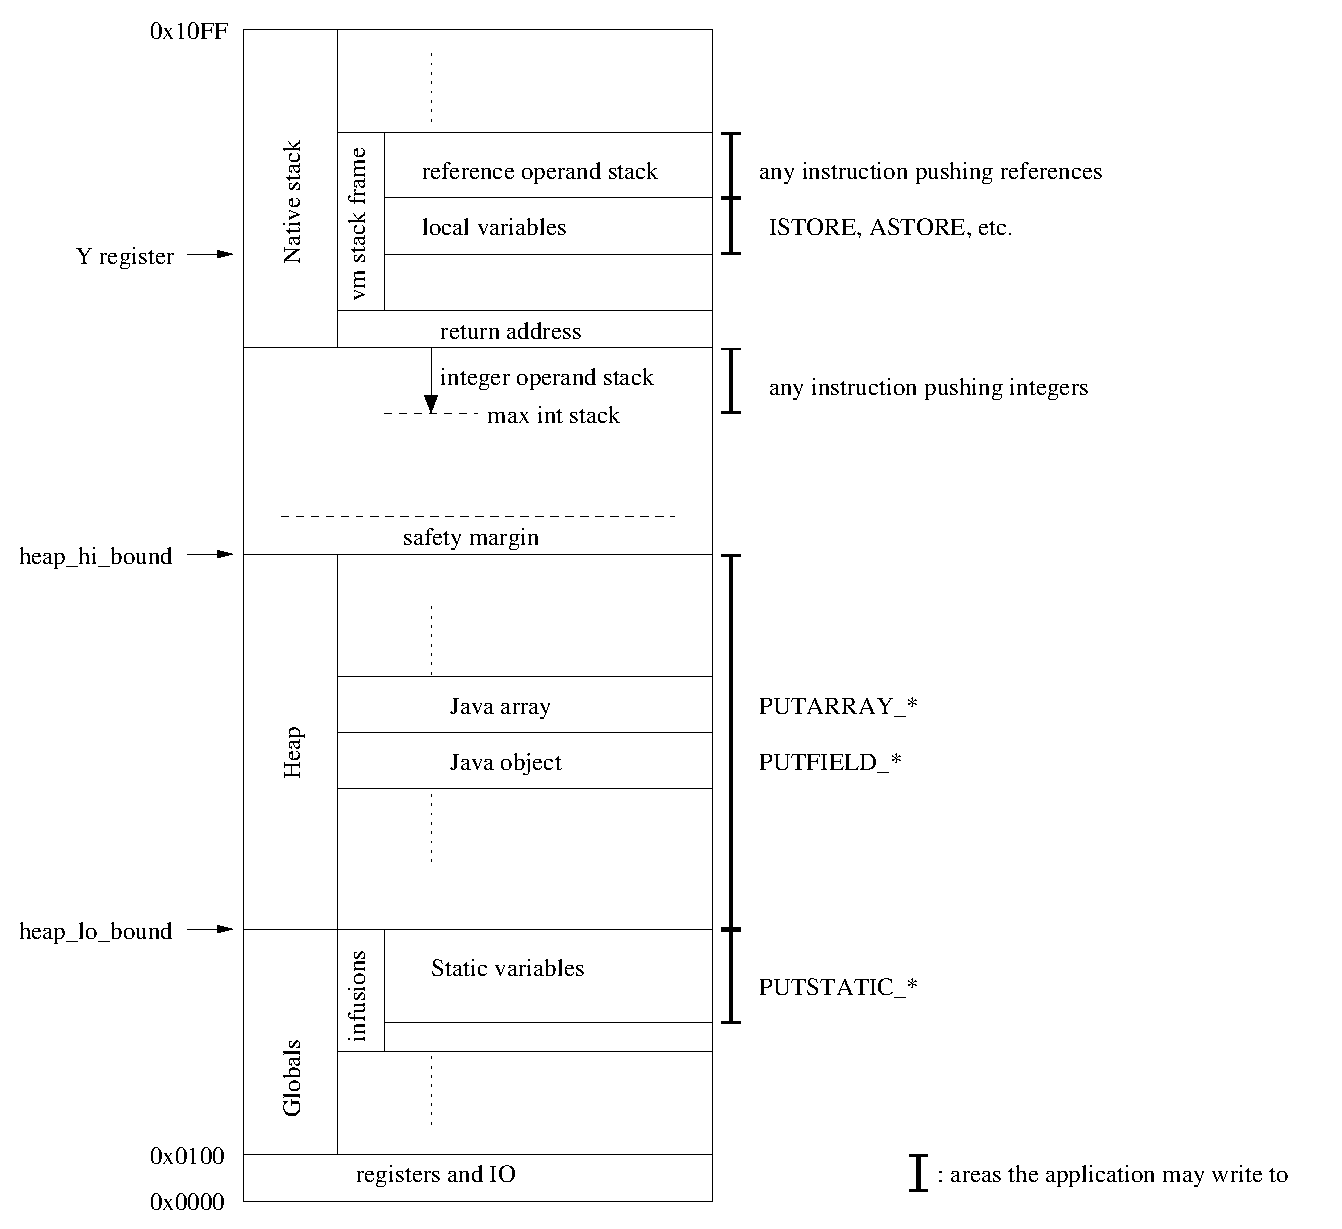
\includegraphics[width=\linewidth]{memlayout.eps}
  \caption{Global memory layout}
  \label{fig-memlayout}
\end{figure}

Figure \ref{fig-memlayout} shows the global layout of the VM's memory. At the bottom are the internal state of by the VM, stored in a number of global variables, and a block with static variables for each infusion. The infusion blocks are actually allocated on the heap at application startup time, but this part of the heap is then separated from the range the application may use to protect them from bad heap writes. This is followed by the application heap, which containts Java objects and arrays.

The native stack grows down in memory towards the heap. This contains a mix of native stack frames for internal VM functions, the application's JVM stack frames containing space for local variables and reference operand stack, and the integer operand stack which grows down directly on the native stack.

This shows how the VM's private data and the application data are mixed in the node's memory. The application is only allowed to write to the areas indicated with bars to the right. Any write outside of these designated areas may corrupt the VM's internal state, and needs to be prevented by our safety checks.

Having ensured control flow safety, we can now rely on the fact that we will always execute complete JVM instructions, and the application cannot skip past an inserted run-time check by jumping to the middle of a generated instruction. This means we can demonstrate memory safety by considering each how each JVM instruction writes to memory, and showing they are all either guaranteed to write to a correct address, or checked at run-time. All JVM instructions can be grouped into one of the categories shown below with respect to their writes to memory.

\begin{table}[H]
\centering
\caption{Instructions writing to memory}
\label{tbl-control-flow-instructions}
\begin{tabular}{ll}
\toprule
type     & writes to \\
\midrule
\mycode{STORE}                   & local variable in stack frame \\
\mycode{PUTSTATIC}               & static variable in infusion \\
\mycode{PUTARRAY}                & heap \\
\mycode{PUTFIELD}                & heap \\
any instruction pushing          & reference or integer stack \\
~~to the stack                   & \\
\bottomrule
\end{tabular}
\end{table}


Since the JVM stack frames are created by the VM based on the method header, we know how much space will be available for local variables and the references stack for normal methods. For lightweight methods, we depend on the caller's stack frame, so we need to make sure this is large enough. Whenever we translate an \mycode{INVOKELIGHT} instruction we verify the stack frame of the current method has reserved enough free space for the lightweight method's locals and stack (\ref{chk-sufficient-stack-space-at-invokelight} and \ref{chk-sufficient-locals-at-invokelight}).

\subsection{The operand stack}
The VM will reserve space for the operand stacks based on the information in the method header, so we need to make sure the actual stack depth neither underflows, or exceeds the maximum announced in the header.

The effect of each instruction on the stack is known at translation time. We simply the verification process by requiring the stack to be empty at all branches, so we can determine the stack depth in a single top to bottom pass. Alternatively, we could announce the expected stack state for each branch target in the method header so we can check the state matches at each branch and corresponding branchtarget. However, this is more complex and in practice the overhead for requiring an empty operand stack at branches is minimal: in all our Java code, only four trivial rewrites to avoid the \mycode{? :} operator were necessary.

This allows us to verify the stack simply by maintaining two counters indicating how many values are on the integer and reference stacks, and updating these counters for each instruction's stack effects as we translate the method. For normal methods both counters are initialised to 0, since they start with empty stacks. Lightweight methods start with their parameters on the stack, so when translating these, the counters are initialised according to the number of arguments announced in the method header.

For each translated instruction, we then check there are enough values on the stack to consume its operands (\ref{chk-no-operandstack-underflow}), and we do not exceed the maximum stack depth announced in the header after pushing it's results (\ref{chk-no-operandstack-overflow}).

Most bytecode instructions have a fixed effect on the stack, for example \mycode{IADD} will always consume two 32-bit ints and push another. We encoded this in a simple table. Method calls, discussed below, require some more work to determine the stack effects. 

\subsubsection{Invoke instructions}
The \mycode{INVOKESTATIC}, \mycode{INVOKESPECIAL}, and \mycode{INVOKELIGHT} instructions all contain the id of the method that will be invoked. We have the method headers for all methods available at translation time, so it is easy to determine the stack effects, since the number of arguments and return value are contained in the header.

For \mycode{INVOKEVIRTUAL} and \mycode{INVOKEINTERFACE} however, the actual method that will be called depends on the object on the stack at run-time. We solve this by choosing the first method implementation that matches the call, and use this method header to determine the stack effects. For valid code all implementations should have the same signature, but malicious code could try to send an implementation in a subclass that has different stack effects. We therefore add a run-time check (\ref{chk-invokevirtual-stack-effects-match}) that will verify the method called at runtime has the same stack effects as the one used to verify the stack at translation time.

\subsubsection{Return}
Note that \mycode{RETURN} instructions don't need any special care. The stack depth will be verified using the instruction found in the bytecode. The return value is passed in registers, so if the return instruction doesn't match the return type in the method header, the result is that either a return value is discarded, or whatever happens to be in registers is used as a return value.

So even though it's possible for a method to break the contract established in the method header, for example by using \mycode{RETURN} instead of \mycode{IRETURN} in a method that should return an int, this can only corrupt the application's own state, and not the VM's.

\subsection{\mycode{STORE}}
Local variable access is easy to verify at translation time. The method header is used to create the current method's stack frame, or for lightweight methods to verify any caller has reserved enough slots for the lightweight method's locals.

Local methods are accessed as an offset from the Y register, which points to the start of the local variables. Since the Y register is controlled by the VM, we only need to check at translation time that the index of the local is within the range announced in the method header to make sure we will write to a valid location (\ref{chk-local-variable-slot-exists}).

\subsection{\mycode{PUTSTATIC}}
Static are allocated globally at the start of the application based on number of static variables in the \emph{infusion} header. The \mycode{PUTSTATIC} instruction contains a reference to an infusion, and the index of the static variable slot. At translation time, we simply need to check the referenced infusion exists (\ref{chk-static-variable-infusion-exists}), and the index is within the legal range (\ref{chk-static-variable-slot-exists}).

\subsection{\mycode{PUTFIELD} and \mycode{PUTARRAY}}
The final type of memory access is to the heap, which happens using the \mycode{PUTFIELD} and \mycode{PUTARRAY} instructions to write to object fields and array elements respectively. The various \mycode{NEW} instructions used to create them are assumed to be safe since they are fully implemented in the VM.

Access to objects and arrays is hard to verify at translation time, without extensive analysis that would be too expensive for a sensor node. For example, a null pointer bug could easily trick the VM to write to the lowest addresses. Since in the AVR, the lowest 32 bytes of the address space are mapped to the CPU's general purpose registers, this can cause very hard to diagnose bugs, as we have experienced first-hand. Similarly, using a high out-of-bounds index into an array, malicious code could easily gain access to the native stack and, for instance, corrupt return addresses.

Here we add a run-time check when translating the instructions just before doing the final memory access to check the address is within the heap (\ref{chk-memory-access-within-heap}).

The VM will set the bounds of the heap in two variables: \mycode{heap\_lo\_bound} and \mycode{heap\_hi\_bound} as shown in Figure \ref{fig-memlayout}. The address to write to is calculated in the AVR's \mycode{Z} register for each heap access instruction. Just before we write to the heap, we insert al \mycode{CALL} to the \mycode{heapcheck} function shown in Listing \ref{lst-heap-bounds-check}.

This function checks the address in \mycode{Z} is within these bounds. If it is not, it will jump to the \mycode{illegal\_access\_handler}, allowing the VM to terminate the application. This check will add 22 cycles overhead for each memory access, and 4 bytes code size overhead for the \mycode{CALL} instruction.

The actual write to the heap is often done by an offset from Z. For example if the offset for an object field is known at compile time, Z is simply loaded with the object's address and the access is done using the correct offset if is less than 64 bytes. If it is higher, Z is first increased to bring it into range.

This means the write could end up at most 63 bytes above the end of the heap, for which we reuse the same small safety margin mentioned in check \ref{chk-no-nativestack-overflow}, which is safe since we will never be writing to a heap object and executing a function in the VM or libc at the same time.

\subsubsection{Alternatives}
We considered several alternative implementations. Since the \mycode{CALL} and \mycode{RET} instruction account for 8 out of these 22 cycles, the checks could be made faster by inlining them. However, inlining would increase the code size overhead from 4 bytes to over 30 bytes, which we considered too high.

We can also save 8 cycles if we keep the bounds in registers instead of memory, which would remove the need for the \mycode{LDS} instructions. However this reduces the performance of the stack cache since it means we have 2 register pairs less for stack caching.

Finally, we could eliminate the need to bounds check the lower byte of the \mycode{Z} register, \mycode{ZL}, if we align the top and bottom of the heap at 256 bytes. This would save 6 cycles, but wastes on average 256 bytes of RAM since some space at the top and bottom of the heap cannot be used.

\begin{listing}[H]
	\centering
 	\begin{minted}{c-objdump}
    heapcheck:
        lds  r0, heap_lo_bound
        cp   ZL, r0
        lds  r0, heap_lo_bound + 1
        cpc  ZH, r0
        brlo illegal_access_handler:
        lds  r0, heap_hi_bound
        cp   r0, ZL
        lds  r0, heap_hi_bound + 1
        cpc  r0, ZH
        brlo illegal_access_handler:
        ret
	\end{minted}
	\caption{Heap bounds check}
	\label{lst-heap-bounds-check}
\end{listing}

%\begin{listing}[H]
%	\centering
% 	\begin{minted}{c-objdump}
%    heapcheck:                               cycles   bytes
%        lds  r0, heap_lo_bound               2        4
%        cp   ZL, r0                          1        2
%        lds  r0, heap_lo_bound + 1           2        4
%        cpc  ZH, r0                          1        2
%        brlo illegal_access_handler:         1        2
%        lds  r0, heap_hi_bound               2        4
%        cp   r0, ZL                          1        2
%        lds  r0, heap_hi_bound + 1           2        4
%        cpc  r0, ZH                          1        2
%        brlo illegal_access_handler:         1        2
%        ret                                  4        2
%	\end{minted}
%	\caption{Heap bounds check}
%	\label{lst-heap-bounds-check}
%\end{listing}
\chapter{Evaluation}
to do

\chapter{Lessons from JVM}
In this chapter we discuss the most pressing issues with current sensor node VMs, summarised in Table \ref{tbl-issues}. We primarily focus on Java, since most of our practical experience is with Java VMs and simplicity of the JVM make it well suited as a basis for sensor node VMs. However, most of the issues we describe also apply to Python, .NET, and other high-level languages.

\begin{table*}
    \centering
    \caption{Point requiring attention in future sensor node VMs}
    \scriptsize
    \label{tbl-issues}
    \begin{tabular}{l|l|l|l}
\hline
\bfseries Sec.              & \bfseries Issue                               & \bfseries in     & \bfseries affects \\
\hline\hline
\ref{sec-std-lib}           & A tailored standard library                   & Standard library & VM size \\
\ref{sec-const-data}        & Support for constant data                     & Java lang., JVM  & memory usage, application size \\
% \ref{sec-small-datatypes}   & Better lang. support for shorts and bytes     & Java lang.       & memory usage, source maintainability \\
\ref{sec-small-datatypes}   & Better lang. support for shorts and bytes     & Java lang.       & memory usage, \\
                            &                                               &                  & ~~  source maintainability\\
\ref{sec-typedef}           & Simple type definitions                       & Java lang.       & source maintainability \\
\ref{sec-inlining}          & Explicit and efficient inlining               & Java lang.       & performance \\
\ref{sec-optimising-javac}  & An optimising compiler                        & javac            & performance \\
\ref{sec-no-gc}             & Allocating objects on stack                   & Java lang., JVM  & (predictable) performance \\
\ref{sec-advanced-features} & Reconsidering adv. language features          & Java lang., JVM  & VM size, complexity, \\
                            & ~~OO, GC, threads, exceptions                 &                  & ~~ and performance \\
%                             &                                               &                  & \\
\hline
\end{tabular}

\end{table*}


\section{A tailored standard library}
\label{sec-std-lib}
\begin{table*}
    \centering
    \caption{Size of Darjeeling VM components}
    \scriptsize
    \label{tab-vm-size}
    \begin{tabular}{l|r|r|cr}
    \hline
    \bfseries Component   & \bfseries std.lib & \bfseries VM & & \bfseries total \\
                          & (bytes)                   & (bytes)              & & (bytes)  \\
    \hline\hline
    core vm               &  3529                     &  7006                & &           10535 \\
    strings               &  8467                     &  1942                & &           10409 \\
    interpreter loop      &     0                     & 10370                & &           10370 \\
    gc                    &    80                     &  3442                & &            3522 \\
    threads               &   909                     &  2472                & &            3381 \\
    exceptions            &  1338                     &   818                & &            2156 \\
    math                  &   222                     &  1274                & &            1496 \\
    io                    &   530                     &   680                & &            1210 \\
    total                 & 15075                     & 28004                & &           43079 \\
     \hline
\end{tabular} 
\end{table*}

A minimum Java APIs for resource constrained devices was proposed by Sun Microsystems, namely the Connected Limited Device Configuration (CLDC) specification \cite{cldc1.1}.  CLDC was primarily intended for larger devices than typical resource constrained sensor nodes.  Providing support for the full CLDC specification would require a substantial amount of memory and program space for features that are rarely required for sensor node applications. Table \ref{tab-vm-size} shows the code size of library support as implemented in the Darjeeling VM \cite{brouwers2009darjeeling}.  Below we outline the most notable features of the CLDC specification that are not necessary for most WSN applications.

String support, which requires a substantial amount of program space, is rarely required within sensor node applications. Although strings may be beneficial during debugging they provide little benefit to application execution. Communication with peripheral hardware is often by means of a stream of bytes. To facilitate such code it would be of benefit to support constant strings at the programming language level (which could be converted to byte arrays under the hood).

A CLDC \mycode{Stream} abstraction is intended to facilitate file, network and memory operations. The abstraction is not well suited for communication protocols required by WSN applications such as I$^{2}$C and SPI. In CLDC, connections between devices can be initiated by specifying URI-like strings. On the other hand, WSN nodes identify other nodes using radio transceiver IDs, typically a 16 or 32-bit identifier.

Other CLDC features that are not required within WSN applications include dynamic class loading, calendar and timezone support.

Other CLDC features that are not required within WSN applications include dynamic class loading, calendar and timezone support. It is clear from the specification that resource constrained WSN applications were not the intended target devices. We argue that a tailored library should be designed from the ground-up specifically for sensor node applications. Such a library would include functionality for: (i) basic math; (ii) array operations; (iii) a communication API that encapsulates the low-level protocols typically used (e.g. I$^{2}$C); and (iv) a higher-level generic radio and sensor API abstraction.

\section{Support for constant data}
\label{sec-const-data}
While Java allows us to declare variables as \mycode{final}, this is only a language level feature, and the VM has no concept of constant data. This is not surprising, since most physical CPUs do not make the distinction either. However, this is different on a sensor node's Harvard architecture where code and data memory are split. The amount of flash memory is usually several times larger than the available RAM, so constant data should be kept in flash instead of wasting precious RAM on data that will never change.

This is especially important for arrays of constant data, which are common in WSN applications. (constant primitive variables are inlined by the compiler, and constant objects are rare) For example our FFT benchmark contains an array of 256 precalculated sine wave values that would be too expensive for the node to calculate at run-time.

When we implement this as a \mycode{final} Java array, the compiler emits a static class initialiser that creates a Java array object, and then uses the normal array access instructions to initialise each element individually:
\begin{minted}{java}
sspush(256);newarray;       // create the array
adup;sconst_0;sconst_0;bastore;  // set index 0
adup;sconst_1;sconst_3;bastore;  // set index 1
adup;sconst_2;bspush(6);bastore; // set index 2
etc...
\end{minted}


There are two problems with this: (i) the array will occupy scarce RAM; and (ii) initialising array elements using JVM instructions requires 4 instructions per element, resulting in 1669 bytes of code to initialise a 256 byte array.

% 
% ####################################### RTC INFUSION bm_fft
%    0     177509286  [avrora.rtc] 3 Start method javax.rtcbench.RTCBenchmark.<clinit> ()V at 0x12e12:    0     201454660  [avrora.rtc] 4  ends at 0x1569a, AOT size: 10376, JVM size: 1669

\textbf{Possible solutions}
Supporting constant arrays will require changes to both the language and bytecode. From the programmer's perspective it should be enough to simply add an annotation like `\mycode{progmem}' to an array declaration to tell the compiler it should be stored in flash. The bytecode will then need to be expanded to allow constant arrays in the constant pool, and to add new versions of the array load instructions (e.g. \mycode{AALOAD} and \mycode{IALOAD}) to read from them.



\section{Better language support for shorts and bytes}
\label{sec-small-datatypes}
Because RAM is scarce, 16-bit short and single byte data types are commonly used in WSN code. The standard JVM only has 32 and 64-bit operations, and variables (instance, local or static) and stack values are stored as 32-bit, even if the actual type is shorter. On a sensor node this wastes memory, and causes a performance overhead since most nodes have 8 or 16-bit architectures, so many sensor node JVMs introduce 16-bit operations and store values in 16-bit slots \cite{brouwers2009darjeeling}.

However, redesigning the VM is only half of the solution. At the language level, Java defines that an expression evaluates to 32-bits, or 64-bits if at least one operand is long. Attempting to store this in a 16-bit variable will result in a `lossy conversion' error at compile time.

As an example, if we have 3 short variables, a, b, and c, and want to do 
\mintinline{java}{a=b+c;}, we need to insert a cast to avoid errors from the Java compiler: \mintinline{java}{a=(short)(b+c);}
% \begin{minted}[fontsize=\footnotesize]{java}
%     a=(short)(b+c);
% \end{minted}

Also, passing literal integer values to a method call treats them as ints, even if they are short enough to fit in a smaller type, which means we end up with calls like: \mintinline{java}{f((byte)1);}
In more complex code that frequently uses of shorts and bytes, these casts can make the code much harder to read.

% Another example from binsrch benchmark:
% mid = (short)((short)(low + high) >>> 1);
% Here we need two cast, the first to avoid compile time error, the second to make sure the infuser uses 16-bit operations instead of 32-bit. But maybe this could be fixed in the infuser, so this is not really a problem with Java

% In C
%   printf("%d\n", 65*4==4);         // => 0
%   printf("%d\n", 1073741825*4==4); // => 1
%   printf("%lu\n", sizeof(1*1));    // => 4


\textbf{Possible solutions}
We suggest that C-style automatic narrowing conversions would make most sensor node code more readable, but to leave the option of Java's default behaviour open, we may implement this as new datatypes: Declaring variable \mintinline{java}{a} as \mintinline{java}{unchecked short} would implictly narrow to short when needed, so \mintinline{java}{a=b+c;} would not need an explicit cast anymore, while declaring it as a normal \mintinline{java}{short} would.

In addition, the server-side component of the split VM should keep intermediate results as shorts where possible. In the example, there's no need to calculate \mintinline{java}{b+c} in 32-bits since the high bits will be truncated anyway.


% If we want to have an efficient sensor node VM, both from a performance and memory usage perspective, better support for data types smaller than 32-bit integers is necessary.
% Java defines that an expression evaluates to the type of its largest operand, or 32-bits, whichever is larger. This automatic expansion to 32-bits could be removed, which means adding two shorts should result in a short value. If we want the result to be 32-bit, we can achieve this by casting one of the operands. Storing a value in a smaller variable should still result in a compile time error, but for the \mycode{a=b+c;} example this would not be necessary anymore, since the result is already a short. In addition, the compiler should treat literal values as the smallest integer type large enough to store it.



\section{Simple type definitions}
\label{sec-typedef}
When developing code for a sensor node, the limited resources force us to adopt different design patterns compared to desktop software. In normal Java code we usually rely on objects for type safety and keeping code readable and easy to maintain. But on sensor nodes, objects are expensive and we frequently make use of shorts and ints for a multitude of different tasks for which we would traditionally use objects.

In these cases we often found that our code would be much easier to maintain if we had a way to name new integer types to explicitly indicate their meaning, instead of using lots of \mycode{int} or \mycode{short} variables. Having type checking on these types would also add a welcome layer of extra safety.

\textbf{Possible solutions}
At a minimum, we should have a way to define simple aliases for primitive types, similar to C's \mycode{typedef}. A more advanced option that fits more naturally with Java, would be to have a strict \mycode{typedef} which also does type checking, so that a value of one user defined integer type cannot be accidentally assigned to a variable of another type, without an explicit cast.



\section{Explicit and efficient inlining}
\label{sec-inlining}
Java method calls are inherently more expensive than C functions. On the desktop, JIT compilers can remove much of this overhead, but on a sensor node we do not have the resources for this. We found this often is a problem for small helper functions that are frequently called. As an example, a C version of the xxtea cipher \cite{wheeler1998xxtea} contains this macro: 
\begin{minted}[fontsize=\footnotesize]{c}
  #define MX (((z>>5^y<<2) + (y>>3^z<<4)) \\
             ^ ((sum^y) + (key[(p&3)^e] ^ z)))
\end{minted}

This macro is called in four places, and is very performance critical. Tools like Proguard \cite{proguard} can be used to inline small methods, but in this case it is larger than Proguard's size threshold. This leaves developers with two unattractive options: either leaving it as a method and accepting the performance penalty, or manually copy-pasting the code, which is error-prone and leads to code that is harder to maintain.

\textbf{Possible solutions}
The simplest solution would be to have a preprocessor similar to C's. However, such a low level text-based solution may not be the most user friendly solution for developers without a C background.
Another option is to give the developer more control over inlining, which could easily be achieved by adding an \mycode{inline} keyword or annotation to force the compiler to inline important methods. These annotations are usually placed at the method level, but since not all calls may be equally important for performance, we may allow the developer to save code space by only inlining certain calls.



\section{An optimising compiler}
\label{sec-optimising-javac}
Java compilers typically do not optimise the bytecode and translate the source more or less as-is. Without a clear performance model it is not always clear which option is faster, and the bytecode is expected to be run by a JIT compiler, which can make better optimisation decisions knowing the target platform and runtime behaviour. However, a sensor node does not have the resources for this and must execute the code as it is received. This leads to significant overhead, for example by repeatedly reevaluating a constant expression in a loop.

\textbf{Possible solutions}
Even without a clear performance model, some basic optimisations can be done. In the experiments described in \cite{reijers2017aot-journal}, some very conservative optimisations already result in code twice as fast as the original.


\section{Allocating objects on stack}
\label{sec-no-gc}
While memory management is too big a topic to cover completely, we do want to mention one relevant observation. In Java anything larger than a primitive value has to be allocated on the heap. This introduces a performance overhead, both for allocating the objects, and the occasional garbage collection run, which may take several thousand cycles.

As an example, one function in the CoreMark \cite{coremark} benchmark uses two small local arrays of 8 ints, which are on the stack in C, but need to be on the heap in Java. In code that frequently needs short-lived objects this overhead can be significant, and unpredictable GC runs are a problem for code with specific timing constraints. In CoreMark's case this adds up to a performance overhead of about 60\% relative to C \cite{reijers2017aot-journal}.

\textbf{Possible solutions}
We suspect it may be possible to avoid this cost in many cases by extending the VM's memory model to allow us to allocate objects and arrays on the stack under certain conditions. We know from TakaTuka's experience that there are many cases where we can determine at compile time that an object can be garbage collected at a certain point \cite{aslam2010optimized}.

If the compiler can determine an object can be freed at the end of the method in which it was created, we can allocate space for it in the method's stack frame. This avoids the overhead of allocating on the heap, and the occasional garbage collection run triggered by this.



\section{Reconsidering advanced language features}
\label{sec-advanced-features}
Finally, we conclude with some discussion on more fundamental language design choices. Many tiny VMs implement some of Java's more advanced features, but we are not convinced these are a good choice on a sensor node.

While features like threads and garbage collection are all useful, they come at a cost. The trade-off when writing sensor node code is significantly different: many of these features are vital to large-scale software development, but the size of sensor nodes programmes is much smaller. And while VM size is not an issue on the desktop, these features are relatively expensive to implement on a sensor node.

In Table \ref{tab-vm-size} we show the code size for some features we discuss below. These were determined by counting the size of functions related to specific features. The actual cost is higher since some, especially garbage collection, also add complexity to other functions throughout the VM. Combined, the features below and the string functions mentioned in Section \ref{sec-std-lib} make up about half the VM.

These features also cause a performance penalty, which is significant when Ahead-of-Time (AOT) compilation is used, and features such as threads and exceptions are much harder in an AOT compiler where we can't implement them in the interpreter loop. This means that if we care about performance and the corresponding reduction in CPU energy consumption, we either have to give them up, or spend considerably more in terms of VM complexity and size.

\subsection{Threads}
As shown in Table \ref{tab-vm-size}, support for threads costs about 10\% of the VM size, if we exclude the string library. In addition, there is the question of allocating a stack for each thread. If we allocate a fixed block, it must be large enough to avoid stack overflows, but too large a block wastes precious RAM. Darjeeling allocates each stack as a linked list of frames on the heap. This is memory efficient, but allocating on the heap is slower and occasionally triggers the GC.

We therefore argue a more cooperative concurrency model is more appropriate where lightweight threads voluntarily yield the CPU and share a single stack.

\subsection{Exceptions}
In terms of code size, exceptions are not very expensive to implement in an interpreter, but again, they are harder to implement in an AOT compiler. We also feel the advantage of having exceptions is much lower than the other features mentioned in this section. They could be easily replaced with return values to signal errors.

\subsection{Virtual methods}
It is hard to quantify the overhead of implementing virtual methods since the code for handling them is integrated into several functions. In terms of size it is most likely less than 2KB, but the overhead for resolving a virtual method call is considerable, and an AOT compiler can generate much more efficient code for static calls.

In practice we seldom used virtual methods in sensor node code, but some form of indirect calls is necessary for things like signal handling. It should be possible to develop a more lightweight form of function pointers that can be implemented efficiently. However, the details will require more careful study.

\subsection{Garbage collection}
Finally, garbage collection is clearly the most intrusive one to change. While the first three features could be changed with minor modifications to Java, the managed heap is at its very core.

Still, there are good reasons for considering alternatives. Table \ref{tab-vm-size} shows the GC methods in Darjeeling add up to about 3.5KB, but the actual cost is much higher as many other parts of Darjeeling are influenced by the garbage collector.

Specifically, it is the reason Darjeeling uses a `split-stack' architecture: the operand stack and variables are split into a reference and integer part. This makes it easy for the GC to find live references, but leads to significant code duplication and complexity. When using AOT compilation, the split stack adds overhead to maintain this state, and the extra register we have to reserve as a second stack pointer.



\section{Conclusion and future work}
In this paper we described a number of issues we encountered over the years while using and developing sensor node VMs. They may not apply to every scenario, but the wide range of the issues we present suggests many applications will be affected by at least some.

Most sensor node VMs already modify the instruction set of the original VM and usually support only a subset of the original language. The issues described here indicate these changes do not go far enough, and we still need to refine our VMs further to make them truly useful in real-world projects.

There are two possible paths to follow: a number of issues can be solved by improving existing Java-based VMs. Staying close to Java also has the advantage of being able to reuse existing knowledge and infrastructure.

However the issues discussed in the last few sections require more invasive changes to both the source language and VM. If the goal is to run platform independent code safely and efficiently, rather than running Java, we should start from the specific requirements and constraints of sensor node software development. We suspect this would lead us to more lightweight features and more predictable memory models.

For either path, we hope the points presented in this chapter can help in the development better future sensor node VMs.

\chapter{Conclusion}


\appendix

\backmatter

\addcontentsline{toc}{chapter}{\bibname}
\bibliographystyle{abbrv}

% Your bibliography goes here
\bibliography{references}

\end{document}
